% Settings for the document is in 'styles/settings.tex'
\documentclass[12pt,a4paper,oneside]{book}
%\usepackage{babel}
\usepackage[utf8]{vietnam}
\usepackage[utf8]{inputenc}
\usepackage{tipa}
\usepackage{amssymb}
\usepackage{graphicx}
\usepackage{subcaption}
\usepackage{booktabs}
\usepackage{mathptmx}
\usepackage{amsmath}
\usepackage{amssymb}
\usepackage{amsfonts}
\usepackage{styles/ipa}
\usepackage{array}
\newcolumntype{P}[1]{>{\centering\arraybackslash}p{#1}}
\newcolumntype{M}[1]{>{\centering\arraybackslash}m{#1}}
\usepackage{fancyhdr}
\usepackage{multirow}
%\usepackage{algorithm2e}
\usepackage{algorithm}
%\usepackage[noend]{algpseudocode}
\usepackage{algpseudocode}
\makeatletter
\renewcommand{\ALG@name}{Giải thuật}
\renewcommand{\listalgorithmname}{Danh sách giải thuật}
\makeatother
% Reinsert missing \algbackskip
\def\algbackskip{\hskip-\ALG@thistlm}
\makeatother
\usepackage{caption}
\captionsetup[algorithm]{labelsep=colon}

% Set line spacing
\linespread{1.2} 
% Set paragraph spacing
\setlength{\parskip}{\baselineskip}%
% Customize hyperlinks
\usepackage{float}
\usepackage{colortbl}
\definecolor{cobalt}{rgb}{0.0, 0.28, 0.67}
\definecolor{carmine}{rgb}{0.59, 0.0, 0.09}
\usepackage[colorlinks=true, urlcolor=carmine, citecolor=cobalt, linkcolor=carmine, pdfborder={0 0 0}]{hyperref}
% Customize algorithm keywords
\usepackage{styles/thesis}
\usepackage{graphicx}
\graphicspath{{figs/}}
\setcounter{secnumdepth}{2}

% Use the followings to skip blank page at the beginning
\usepackage{atbegshi}% http://ctan.org/pkg/atbegshi
\AtBeginDocument{\AtBeginShipoutNext{\AtBeginShipoutDiscard}}

% For code highlighting
\usepackage{minted}

% Input thesis information
\crname{ĐỒ ÁN TỐT NGHIỆP ĐẠI HỌC}
% Nhập tên đồ án 
\ctname{TÌM HIỂU THƯ VIỆN PYTORCH,\\ỨNG DỤNG XÂY DỰNG HỆ THỐNG NHẬN DẠNG LOÀI VẬT QUA ẢNH}
% Họ và tên SV, MSSV
\cstuname{Lê Trọng Kha (60135804)}
% Tên ngành
\csCouncil{Công nghệ thông tin}
% Họ và tên GV hướng dấn
\csSupervise{TS. Nguyễn Đình Hưng}
% Năm thực hiện đồ án
\cttime{2022}
% Set thesis layout (defined in 'thesis.sty')
\thesislayout

\begin{document}
% Add cover page to the document (defined in 'styles/thesis.sty')

\coverpage

% The \frontmatter command makes the pages numbered in lowercase roman, and makes chapters not numbered
\frontmatter

% Declaration page
\begin{declaration}
Tôi xin cam đoan đây là công trình nghiên cứu của riêng tôi dưới sự hướng dẫn của...Nếu phát hiện có bất kì sự gian lận nào, tôi xin hoàn toàn chịu trách nhiệm về nội dung đồ án của mình.
\end{declaration}

\newpage

% Acknowledgement page
\begin{acknowledgments}
Tôi xin chân thành biết ơn thầy X đã hướng dẫn tận tình trong suốt quá trình thực hiện Đồ án tốt nghiệp này.


Tôi xin bày tỏ lòng biết ơn sâu sắc nhất đến ba mẹ tôi...

\end{acknowledgments}

% Abstract page
\begin{abstract}
Đồ án này nhằm tìm hiểu các phương pháp và kỹ thuật tiên tiến của Trí tuệ nhân tạo và ứng dụng vào bài toán nhận dạng loài vật qua ảnh.
\end{abstract}	

% Bảng mục lục
\tableofcontents
% Danh mục bảng
\listoftables
% Danh mục hình
\listoffigures
% Danh mục giải thuật
\listofalgorithms

\mainmatter
\fancyhead{}  % Clears all page headers and footers
\renewcommand{\footrulewidth}{0.4pt}
\pagestyle{fancy} 
\renewcommand{\chaptermark}[1]{\markboth{#1}{#1}}
\fancyhead[R]{\chaptername\ \thechapter\ --\ \leftmark}

\chapter {Giới thiệu}\label{chapter_1}
	
\section{Đặt vấn đề}
\subsection{Sự phát triển của Trí tuệ nhân tạo và Học máy}
Nhập nội dung của subsection ở đây.
Trích dẫn \cite{Krizhevsky2012}.
\subsection{Ứng dụng Học máy xây dựng hệ thống nhận dạng hình ảnh}
Nhập nội dung của subsection ở đây.

\section{Mục tiêu của đề tài}

Các mục tiêu chính của đề tài bao gồm:
\begin{itemize}
\item Tìm hiểu tổng quan về Trí tuệ nhân tạo và ứng dụng;
\item Tìm hiểu cơ sở toán học và mô hình học máy;
\item Xây dựng hệ thống nhận dạng loài vật tự động qua ảnh, sử dụng mô hình học máy tiên tiến;
\item Triển khai mô hình thành ứng dụng.
\end{itemize}

\section{Cấu trúc của Đồ án}
Đồ án gồm các phần như sau:
\begin{itemize}
\item Chương 1: Giới thiệu. 
\item Chương 2: Các kiến thức nền tảng.
\item Chương 3: Tổng quan một số công trình nghiên cứu liên quan tới đề tài.
\item Chương 4: Trình bày hướng tiếp cận giải quyết bài toán. Mô tả thực nghiệm và phân tích, nhận xét kết quả.
\item Chương 5: Kết luận.
\end{itemize}
\chapter{Tổng quan}\label{chapter_2}

Phần dẫn nhập của Chương \ref{chapter_2}.

Chuyển sang Chương \ref{chapter_1}.

\section{Chèn hình ảnh}

Hình \ref{icc_plot} minh họa chèn hình ảnh vào báo cáo.
 
\begin{center}
    \begin{figure}[h!]
    \begin{center}
     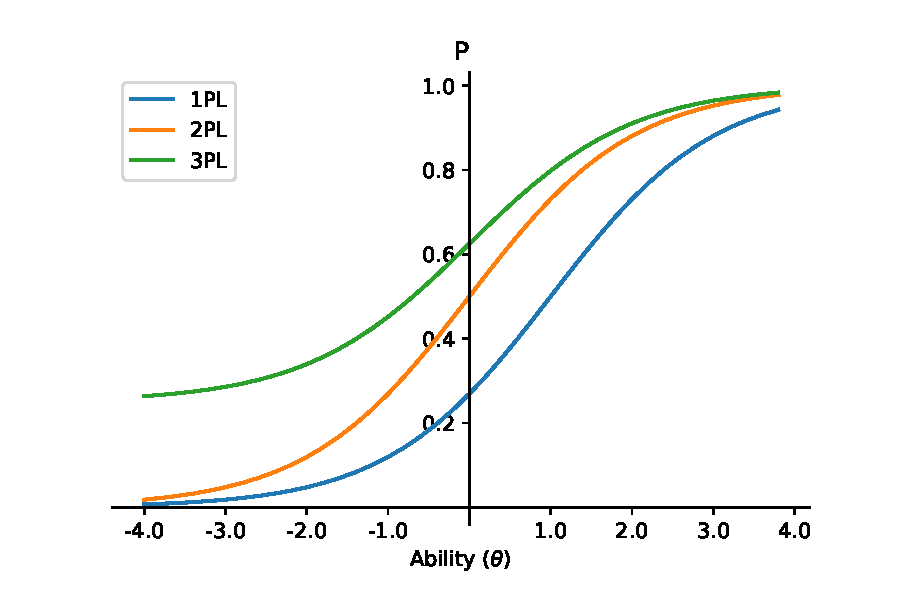
\includegraphics[scale=0.5]{figs/ICC_plots.pdf}
    \end{center}
    \caption{Một ví dụ về chèn hình ảnh.}
    \label{icc_plot}
    \end{figure}
\end{center}

\section{Chèn bảng}

\begin{center}
    \begin{table}
    \centering
    \caption{Ví dụ về tạo bảng trong \LaTeX. Tham khảo: \url{https://en.wikibooks.org/wiki/LaTeX/Tables}.}
        \begin{tabular}{ |l|l|l| }
        \hline
        \multicolumn{3}{ |c| }{Danh sách U23 Việt Nam tại Sea Games 31} \\
        \hline
        Thủ môn & GK & Nguyễn Văn Toản \\ \hline
        \multirow{4}{*}{Hậu vệ} & LB & Phan Tuấn Tài \\
         & DC & Bùi Hoàng Việt Anh \\
         & DC & Lê Văn Đô \\
         & RB & Lê Văn Xuân \\ \hline
        \multirow{3}{*}{Tiền vệ} & MC & Đỗ Hùng Dũng \\
         & MC & Nguyễn Hoàng Đức \\
         & MC & Dụng Quang Nho \\ \hline
        
        \multirow{2}{*}{Tiền đạo} & ST & Nhâm Mạnh Dũng \\
         & ST & Nguyễn Văn Tùng \\
         & FW & Nguyễn Tiến Linh \\
        \hline
        \end{tabular}
    
    \end{table}
\end{center}

\section{Chèn công thức toán học}

Công thức \ref{eq:InterTweetInteraction} thể hiện mức độ tương tác giữa hai tập $T_{j}^{P}$ và $T_{k}^{P}$.

\begin{align}
S_{j,k}^{P}=\frac{\sum_{t_{m}^{P}\in T_{j}^{P}}\sum_{t_{n}^{P}\in T_{k}^{P}}r\left(t_{m}^{P},t_{n}^{P}\right)}{|T_{j}^{P}||T_{k}^{P}|}\label{eq:InterTweetInteraction}
\end{align}\label{formula_1}

\section{Chèn mã nguồn}
Có thể sử dụng package minted để chèn mã nguồn vào báo cáo. Có thể chèn mã nguồn trực tiếp hoặc từ file có sẵn.

\noindent\textbf{Ví dụ 1:} Chèn mã nguồn trực tiếp.
\begin{minted}{C++}
#include<stdio.h>
int main()
{
	printf("Hello world!");
}
\end{minted}


\newpage
\noindent\textbf{Ví dụ 2:} Chèn mã nguồn từ file.
\inputminted{c++}{code/XulyFileText.cpp}

\section{Biểu diễn giải thuật}

    \begin{algorithm}[H]
    \caption{Kiểm tra một số tự nhiên có phải số nguyên tố hay không}\label{prime_number_check}
    \hspace*{\algorithmicindent} \textbf{Input:} 
    Số tự nhiên \textbf{n}
    \\
    \hspace*{\algorithmicindent} \textbf{Output:} 
    True nếu \textbf{n} là số nguyên tố,
    False nếu \textbf{n} không phải số nguyên tố
    \begin{algorithmic}[1]
    \Function{isPrimeNumber}{n}
    \If {$n < 2$} \Return False
    \EndIf
    \For{$i \gets 2$ to $n/2$}
    \If{$n \% i == 0$} \Return False
    \EndIf
    \EndFor
    \State \Return True
    \EndFunction
    \end{algorithmic}
    \end{algorithm}





\chapter{Convolutional Neural Networks}

\section{Giới thiệu}
\input{chapters/chapter4-thucnghiemvadanhgia}
\chapter{Kết luận}

\section{Những kết quả đạt được}

\section{Một số hạn chế và hướng phát triển của đề tài}

% Tài liệu tham khảo
\bibliographystyle{plain} 
\bibliography{refs}

% Kết thúc
\end{document}